%%% LaTeX Template
%%% This template can be used for both articles and reports.
%%%
%%% Copyright: http://www.howtotex.com/
%%% Date: February 2011

%%% Preamble
\documentclass[paper=a4, fontsize=11pt]{scrartcl}	% Article class of KOMA-script with 11pt font and a4 format

\usepackage[margin=0.7in]{geometry}
\setcounter{secnumdepth}{4}

\usepackage[english]{babel}															% English language/hyphenation
\usepackage[protrusion=true,expansion=true]{microtype}				% Better typography
\usepackage{amsmath,amsfonts,amsthm}										% Math packages
\usepackage[pdftex]{graphicx}														% Enable pdflatex
\usepackage{seqsplit}
%\usepackage{color,transparent}													% If you use color and/or transparency
\usepackage[hang, small,labelfont=bf,up,textfont=it,up]{caption}	% Custom captions under/above floats
\usepackage{epstopdf}																	% Converts .eps to .pdf
\usepackage{subfig}																		% Subfigures
\usepackage{booktabs}																	% Nicer tables


%%% Advanced verbatim environment
\usepackage{verbatim}
\usepackage{fancyvrb}
\DefineShortVerb{\|}								% delimiter to display inline verbatim text


%%% Custom sectioning (sectsty package)
\usepackage{sectsty}								% Custom sectioning (see below)
\allsectionsfont{%									% Change font of al section commands
	\usefont{OT1}{bch}{b}{n}%					% bch-b-n: CharterBT-Bold font
%	\hspace{15pt}%									% Uncomment for indentation
	}

\sectionfont{%										% Change font of \section command
	\usefont{OT1}{bch}{b}{n}%					% bch-b-n: CharterBT-Bold font
	\sectionrule{0pt}{0pt}{-5pt}{0.8pt}%	% Horizontal rule below section
	}


%%% Custom headers/footers (fancyhdr package)
\usepackage{fancyhdr}
\pagestyle{fancyplain}
\fancyhead{}														% No page header
\fancyfoot[C]{\thepage}										% Pagenumbering at center of footer
\renewcommand{\headrulewidth}{0pt}				% Remove header underlines
\renewcommand{\footrulewidth}{0pt}				% Remove footer underlines
\setlength{\headheight}{13.6pt}

%%% Equation and float numbering
\numberwithin{equation}{section}															% Equationnumbering: section.eq#
\numberwithin{figure}{section}																% Figurenumbering: section.fig#
\numberwithin{table}{section}																% Tablenumbering: section.tab#
\usepackage[parfill]{parskip}
\usepackage{float}
\usepackage{graphicx}
\usepackage{hyperref}
\usepackage[numbers]{natbib}

\newcommand{\sectionbreak}{\clearpage}


%%% Title
\title{ \vspace{-1in} 	\usefont{OT1}{bch}{b}{n}
		\huge \strut CS32310: A Virtual Orrery\strut \\
}
\author{ 									\usefont{OT1}{bch}{m}{n}
        Samuel Jackson\\		\usefont{OT1}{bch}{m}{n}
		Department Of Computer Science\\	\usefont{OT1}{bch}{m}{n}
        Aberystwyth University\\
        \texttt{slj11@aber.ac.uk}
}
\date{\today}

%%% Begin document
\begin{document}
\maketitle

\section{Introduction}
This report documents the CS32310 Advanced Graphics assignment. The task for this assignment was to build a virtual orrery of the solar system using WebGL, HTML5, and Javascript. The finished implementation presented here has both the basic functionality outlined in the assignment brief (i.e. drawing, texture mapping, lighting, and animating spheres) along with some non-trivial additional functionality such as multi-texturing, elliptical orbits, and transparency. 

All of the files required for this project are supplied in the requested zip folder. Additionally, after the assignment deadline has passed, I will make the code for this project publicly available from github \cite{github} and running the simulation will be accessible via a public Github pages branch, The project files provided in the zip folder should be run from a HTTP web server if the user is looking at this locally using the Chrome browser. This is because Chrome disables loading local files by default which will cause an error and the WebGL application will be unable to run. Running a local Python server from the command line is the easiest way to achieve this.

The first section of this report outlines the basic functionality and overall structure of the application produced while the second section outlines the more advanced features implemented in the application. The final section concludes the report with a brief description of the problems I encountered throughout the assignment and what I would of done differently with hindsight.

\section{Basic Implementation}
In this assignment I have heavily relied upon Javascript objects and prototypes to implement most of the functionality for the project. As Javascript has no support for classes, I have simulated classes by using objects with methods and attributes added to the prototypes which can be accessed using the \textit{this} keyword. Copies of an object can be created using the Javascript \textit{new} keyword. To simulate inheritance, I have used a small utility function called \textit{extends} which copies the prototype of a parent to a child.

\subsection{Models}
In my implementation I have created a collection of model objects that define how something that is drawable in the scene should look and how it should be positioned. This is achieved using a hierarchy of extended prototypes, each adding additional functionality to the previous one. The most basic of these models is the Drawable object. This has very little implementation and only defines some common functions and attributes that are shared between all models. These include initialising the vertex, texture, index, and normal buffers, drawing the buffers, setting the drawable object's position etc. From this model two slightly more complex models are defined called Sphere and Cube. Unsurprisingly these have constructor functions which create vertex, index, texture, and normal data for objects that are spherical and cubic respectively.

\begin{figure}[H]
\centering
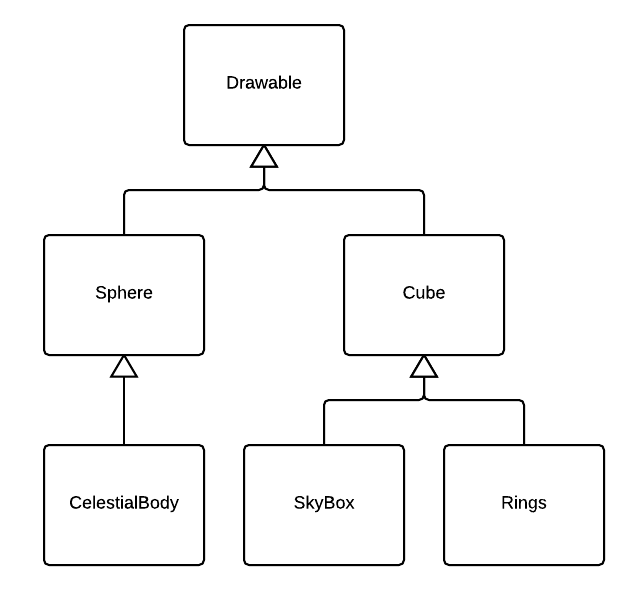
\includegraphics[width=0.5\textwidth]{img/model-uml.png}
\caption{UML diagram of the hierarchy of ``inheritance'' of prototypes for models in the  application.}
\label{fig:uml-models}
\end{figure}

From these basic model definitions several other models are defined, the most important being the CelestialBody object. This object extends the Sphere model to include methods and attributes for positioning and texturing a celestial body such as the sun, earth or moon. This includes the code for modifying the model-view matrix to correctly position and animate the celestial body based on parameters defining its orbit, axis rotation, texture etc.

Alongside the CelestialBody object there are several other models defined which are used in the simulation. The SkyBox model extends the Cube model's prototype to add functionality for drawing a large cube with a cube map texture attached. This is used give the illusion that the scene has a background in the distance. Another model used in the Rings model. This is another extension of the cube model used to define how transparent rings such as the rings of Saturn are positioned and displayed within the scene.

\subsection{Controlling the Scene}
Controlling the scene is handled by an object call the SceneGraph. This controls in what order drawable objects in the scene should be drawn from a list of drawables. CelestialBody objects have a list of objects that orbit them. In order to correctly position them within the scene the scene graph effectively performs a post order traversal. The scene graph first applies transformations that should affect both the current drawable item and all of its children, then processes any children, then transforms and draws the current item. Children are passed a copy of the model-view matrix with any global transforms applied so that the parent models are unaffected by the transformation of their children.

In a similar way, the scene graph is also responsible for calling the animate function on every model in the tree and for traversing the tree to initialise the buffers of every model. The scene graph is also responsible for building a tree of drawable objects for a loaded JSON configuration file. The scene graph also has some limited support for a transparency buffer (see section \ref{sec:advanced-features}).

\subsection{Textures}
The textures used throughout the program are loaded in a separate Javascript object called the TextureLoader. This iterates over a dictionary of textures that defines the name of the texture as the key and the location of the file as the value. A new dictionary is created using the keys of the original but with the value of the loaded texture. If the value of an item in the original dictionary is not one file path but a list of file paths the TextureLoader assumes that this is a cube map and will load it as such. The returned dictionary is stored with global access within the program which allows access to the loaded textures when the drawable objects are drawn. Note that only one copy of every texture is ever loaded and this is shared between multiple uses of the texture, such as the texture for the moons.

\subsubsection{Shaders}
I have implemented two different shader programs for this assignment. The first and main one is the shader which is used to render the sun, planets and moons in the solar system. This shader program also adds support for a full Phong shading lighting model within the fragement shader. This shader also has support for multi-texturing and light attenuation (see section \ref{sec:advanced-features}).

\begin{figure}[H]
\centering
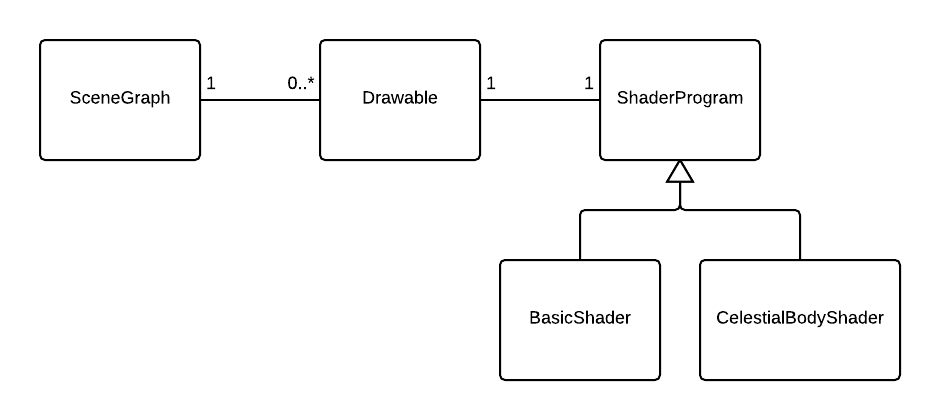
\includegraphics[width=0.8\textwidth]{img/shader-uml.png}
\caption{UML class diagram showing the relationship between the SceneGraph, Drawables, and the Javascript shader programs.}
\label{fig:shaders-uml}
\end{figure}

The second shader is much more basic. This is just used to render the cube mapped sky box (see section \ref{sec:advanced-features}) with an ambient lighting term. This was because the sky box should be unaffected by the directional lighting emitted by the sun. Having a different shader program reduces the load on the fragment shader because less parameters need to be passed in order to set-up and render with the shader and there are hardly any operations at either the vertex or fragment shader level.

To accompany these two shader programs there are two Javascript objects which set-up all of the shader uniforms prior to drawing a model. Each of these Javascript shader objects are passed a dictionary of shader uniforms that apply globally to all objects drawn with this shader program upon instantiation. Each instance of a model object stores a dictionary of uniforms that are applicable to that specific object. These individual uniforms are passed to the shader program object before drawing the model so that the specific configuration for the current drawable object is correctly set-up beforehand. Both of the Javascript shader objects are stored in a global object called shaders.

\subsection{Cameras and Control}
A Javascript object called SphericalCamera is used to control the current position of the perspective matrix. This listens for input from the user from the keyboard according to a predefined list of key commands (see section \ref{sec:controlling-the-simulation}). This is implemented using a spherical coordinate system. The camera has a reference to a CelestialBody which it is currently focussed on. The camera uses the position of the focused CelestialBody to determine the direction that the camera should be looking using the glMatrix library \textit{lookAt} function. Keyboard commands are listened to in an object called the KeyController. This listens for keyboard events from the user before calling the callback functions for the camera.

\section{Advanced Features}
\label{sec:advanced-features}
Alongside the basic functionality requested by the assignment brief, I have also implemented an number of additional features to extend the simulation further. This section documents these additional features and discusses how they're implemented within the project.

\subsection{Light Attenuation}
One of the simplest additional features I have included is light attenuation. As the distance from the point light position (the sun) is increased, the intensity of the lighting upon a sphere is penalised by an additional coefficient calculated in the fragment shader code.  The attenuation of the light source is calculated using three supplied coefficients in a  quadratic term given by the equation:

\begin{equation}
\frac{1}{c_1 + c_2r + c_3r^2}
\end{equation}

Where $c_1$,$c_2$, and $c_3$ are the supplied coefficients and $r$ is the distance from the light source. In the simulation for this assignment, these terms can be adjusted using the control panel and are set to sensible defaults that should illuminate every planet in the system by at least a small amount.

\subsection{Rings of Saturn}
The next additional feature that I have implemented in this assignment is to create the rings of Saturn using the RGBA texture provided. The implementation uses the alpha information provided in the texture together with the blending functionality provided by WebGL to make the rings appear ``see through''. To accomplish this effect I created a very thin texture mapped cube and created a new extension of the Cube model called Rings. 

\begin{figure}[H]
\centering
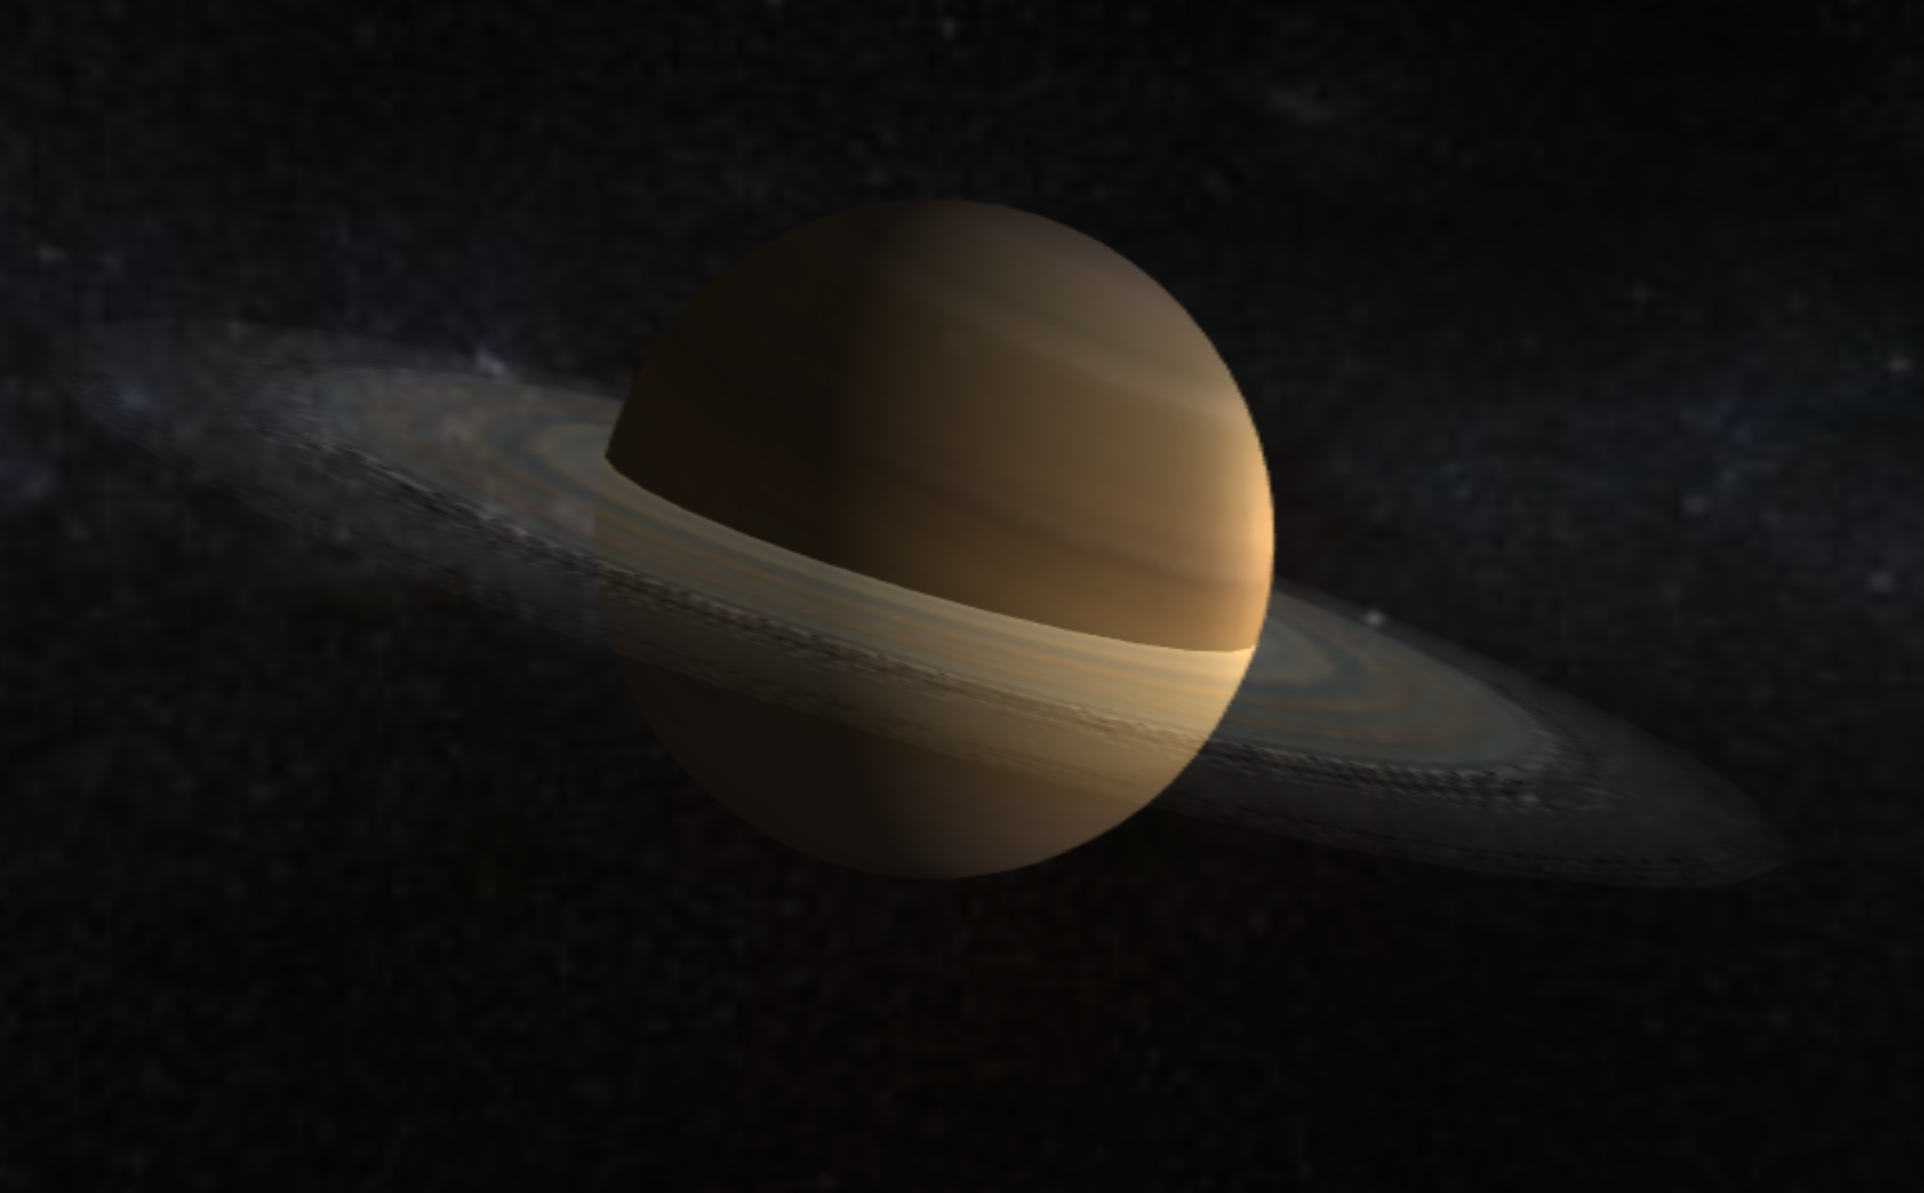
\includegraphics[width=0.5\textwidth]{img/saturns_rings.png}
\caption{Saturn's rings with transparency and blending.}
\label{fig:saturns-rings}
\end{figure}

An additional parameter indicating whether a drawable item should be blended was also added to the prototype of the Drawable object so that the scene graph knows that this item must be drawn after the others. Instead of being drawn as the scene graph traverses the tree a blended object is added to a separate buffer so that it can be processed after all of the non-blended objects have been drawn in the scene. This buffer is just implemented as a Javascript list which is iterated over and the objects inside are drawn with blending turned on and with the appropriate blending function set. To ensure that the objects are still positioned correctly, objects in the blending buffer are stored alongside a copy of the correct version the model-view matrix that should be used to transform them.

Currently the rings of Saturn are the only object that exists in the scene that needs to be drawn using transparency. If there were other items in the scene that needed drawing they would be drawn in the order in which they appear during the traversal of the scene graph from the buffer described above. This would cause incorrect rendering of the scene as no information about the z position of the blended object relative to the camera is used to sort the blending buffer prior to drawing. This is discussed in the next section as an area for future improvement.

\subsection{Elliptical Orbits}
Another feature that I have implemented in this project is elliptical orbits for the planetary bodies using Kepler's first two laws of orbital motion. Parameters for the constants of angular velocity and eccentricity can be set as options during the creation of a CelestialBody. The orbital radius parameter describes the starting point of the body relative to the centre of the body that it orbits; in the case of the sun this is just the origin. Correct positioning is handled as part of the scene graph where a body orbiting a planet first has all of its parent's transformations applied and then adjusts the model view matrix to position itself. This is extremely useful as it means that the radius of a planet's orbitals do not need to be changed when the position of the planet changes.

\begin{figure}[H]
\centering
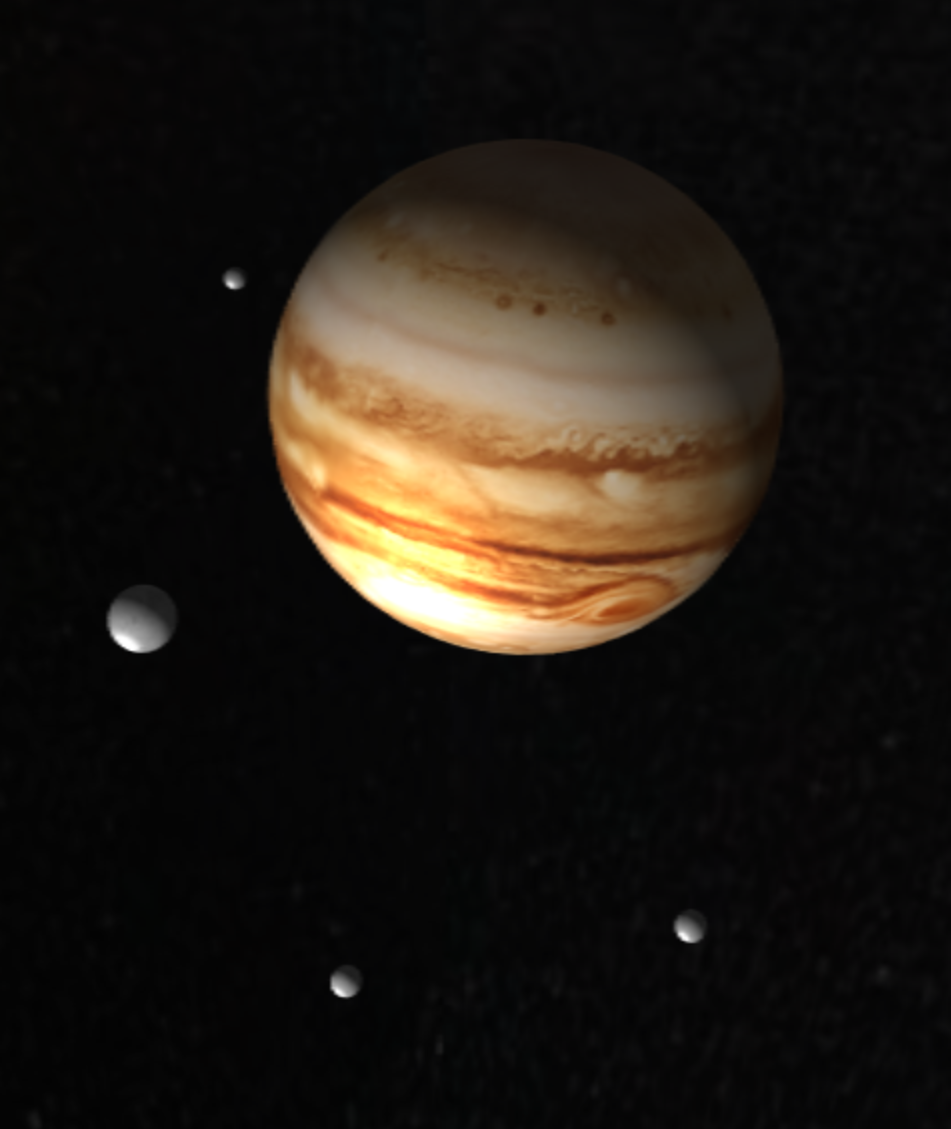
\includegraphics[width=0.4\textwidth]{img/jupiter_moons.png}
\caption{Jupiter with four moons in elliptical orbits.}
\label{fig:jupiter-moons-elliptical}
\end{figure}

\subsection{Multi-texturing}

\subsubsection{Earth's Atmosphere}
I have used two different types of multi-texturing to make the earth appear more realistic. The first use of multi-texturing was to use another texture for the atmosphere of earth. This is supplied as a few additional parameters to the shader. One indicates if a  cloud texture is being used, one for the texture itself and one specifying the current rotation of the atmosphere texture about the surface of the planet.

If a texture for the atmosphere is supplied to a CelestialBody, the texture is sampled in the fragment shader using the current texture coordinates passed from the vertex shader, but with the current x position rotated by the parameter specifying the current position of rotation of the atmosphere about the earth's surface. This gives the effect that the atmosphere is rotating independently to the rotation of the earth. Updating the current position of the atmosphere's rotation is calculated in the animate method in the CelestialBody object and the speed of the rotation is a configurable parameter. The alpha information in the texture for the atmosphere is then weighted according to the equation:

\begin{equation} \label{eq:transparent-texture}
I = (1-a)I_1 + aI_2
\end{equation}

Where $I_1$ is the sampled texture of the earth, $I_2$ the sampled texture of the atmosphere, and $a$ is the alpha information from the atmosphere. This weights the sampled texture colour so that the non-transparent clouds appear instead of the earth texture but still allow the texture of the earth to show through where there are no clouds.

\begin{figure}[H]
\centering
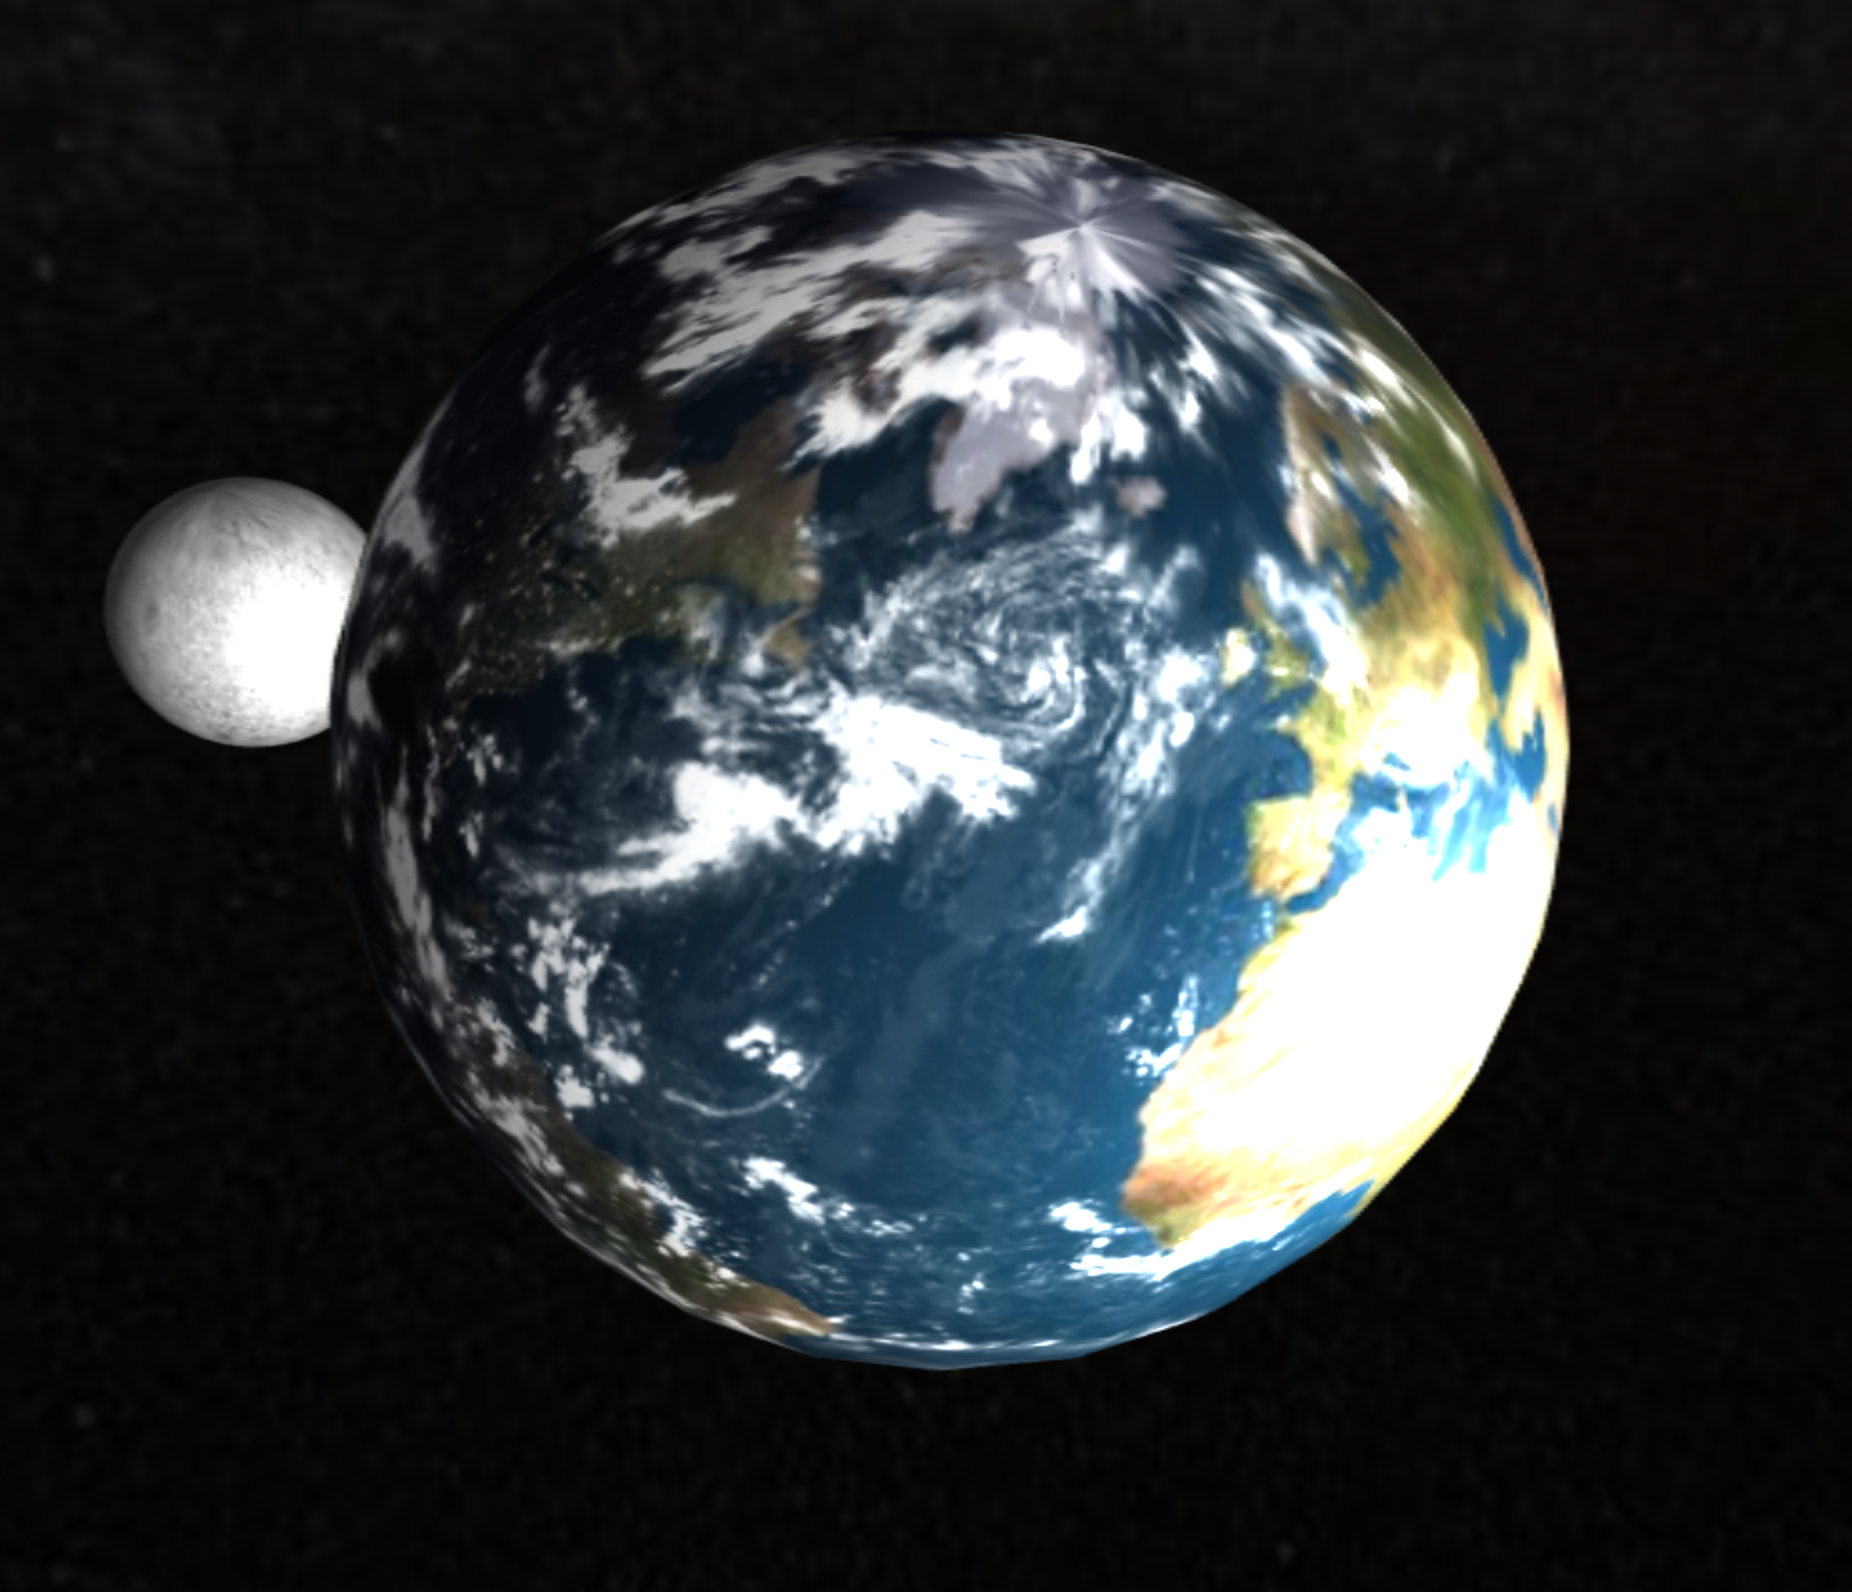
\includegraphics[width=0.6\textwidth]{img/earth.png}
\caption{Earth with multi-textured atmosphere. The night lights on the dark side of the earth can just be made out on the left side of the earth in this image.}
\label{fig:earth-multi-texture}
\end{figure}

\subsubsection{Dark Side of the Earth}
The second use of multi-texturing is the use of a night texture for the dark side of the earth. This texture shows the earth at night as a dark blue texture with lights positioned at the major cities on the planet. As the earth rotates about its axis the day time texture slowly transforms into the night texture, giving the appearance of the lights of the major cities appearing as the earth rotates away from the sun. 

To achieve this effect an additional two parameters were supplied to the shader, one for whether a dark texture should be used and one for the dark texture itself. If a dark texture is used the dark texture is sampled using the same coordinates that are used for the light texture. The amount of information from each texture is then weighted using the same equation as \ref{eq:transparent-texture} but with the atmosphere alpha information replaced by the factor for the amount of diffuse lighting at this fragment and the atmosphere texture replaced by the dark side texture. This means that both the light and dark textures for the earth's surface are sampled proportionally to the amount of light falling on a fragment.

\begin{figure}[H]
\centering
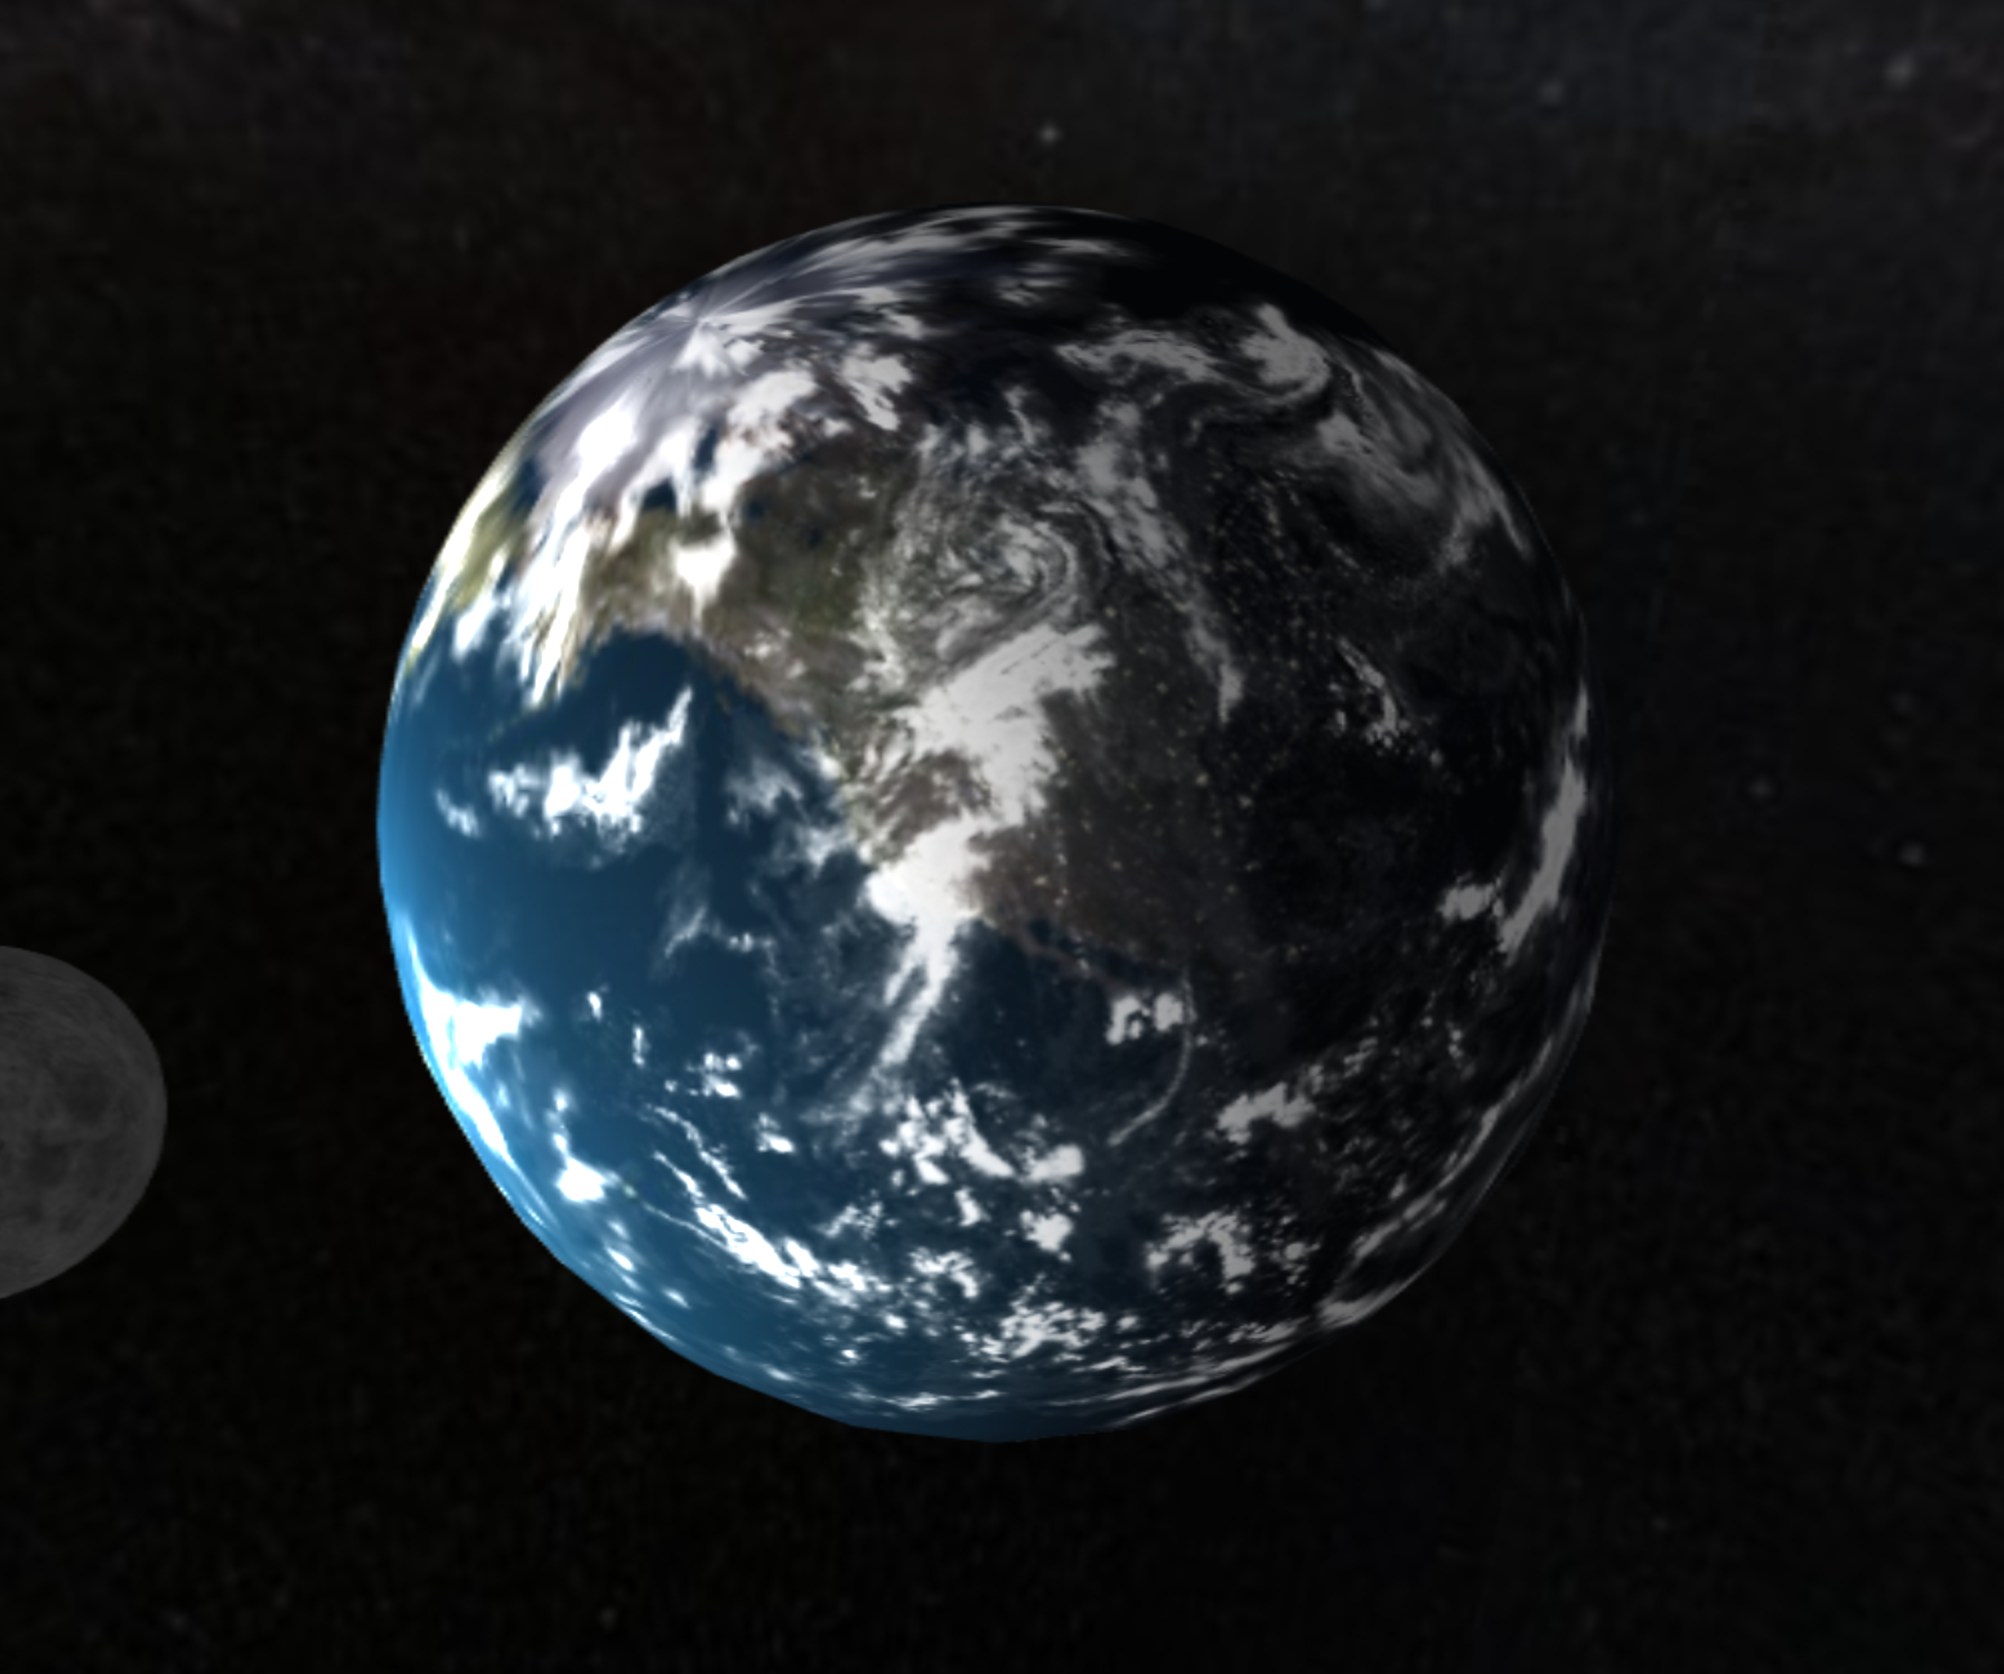
\includegraphics[width=0.6\textwidth]{img/earth_dark.png}
\caption{Slightly better shot of the dark texture on earth. The night lights can be seen to the right of the screen shot over north America.}
\label{fig:earth-dark}
\end{figure}

\subsection{Cube Mapped Background}
One final minor feature that I have added to the simulation is a cube mapped background which is textured to look like a picture of our galaxy. This background is created by using six different images; one for each face of the cube. The images are then loaded and assigned the correct position in the cube map texture. This texture is then applied to a very large cube drawn around the scene giving the appearance of the solar system being within a galaxy. This cube is drawn with a completely different shader program from the one used by the solar system. This is because the cube map only requires a constant ambient lighting term and should not be affected by directional lighting which would also impact efficiency as much larger number of fragment shader operations would have to be performed.

\section{Controlling the Simulation}
\label{sec:controlling-the-simulation}
As part of the simulation I have implemented a basic control panel that allows the user to control some aspects of the scene. I have also included a camera that can be used to move around the simulation and look at different planets.

\subsection{Control Panel}
Upon starting the simulation a control panel will be visible on the right hand side of the page. The panel gives a brief listing of the controls that can be used within the application and also has options to adjust parameters controlling the lighting in the scene. The options for controlling the scene are listed as follows:

\begin{table}[H]
\centering
\begin{tabular}{ l p{12cm}}
Key Command & Action \\ \hline
\textit{Q} & Open/Close the control panel \\ \hline
\textit{W} & Zoom in on the currently selected planet \\ \hline
\textit{S} & Zoom out from the currently selected planet \\ \hline
\textit{Arrow Keys} & Move the camera around the currently selected planet \\ \hline
\textit{F1-10} & Change the currently selected planet \\ \hline

\end{tabular}
\caption{Table listing the key commands that are used in the simulation.}
\label{table:keyboard-controls}
\end{table}

The control panel lists five configurable options to do with the lighting of the scene. The parameters that each of these options controls are listed in the following table:

\begin{table}[H]
\centering
\begin{tabular}{ l p{12cm}}
Control & Description \\ \hline
\textit{Intensity} & Uniformly increases/decreases the RGB values for the point light colour \\ \hline
\textit{Shininess} & Increases/decreases the material shininess of the specular lighting\\ \hline
\textit{Constant attenuation} & Sets the value of the constant term of light attenuation \\ \hline
\textit{Linear attenuation} & Sets the value of the linear term of light attenuation \\ \hline
\textit{Quadratic attenuation} & Sets the value of the quadratic term of light attenuation \\ \hline

\end{tabular}
\caption{Table listing the lighting controls that are used in the simulation.}
\label{table:lighting-controls}
\end{table}

\subsection{Camera Control}
The camera uses the glMatrix library \textit{lookAt} function to generate a matrix that is always looking at the center of a planet. The arrow keys (see table \ref{table:keyboard-controls}) can be used to rotate around the planet along two axes. When looking at a planet other than the sun the camera will move with the planet's orbit so that the viewer may gain a decent view of the planet as it moves. When swapping between planets the zoom distance is automatically reset to a distance that is proportional to the radius of the currently selected planet. This is to ensure that the camera does not end up starting inside a larger planet or very far way from a smaller one.

\section{Conclusion}
\label{sec:conclusion}
In conclusion, I would like to outline some areas where I encountered problems along the way, some of the things which I felt worked well, and some suggestions for further improvements upon the existing work. 

One area of the project which I felt worked quite well was the use of a tree like structure for the organisation of planets. This meant that the correct model-view matrix could be applied to each planet and have the parent planet's transforms applied to it at the same time, but also prevented the incorrect transformation from being applied to a planet as a copy could be made and passed to the children, so the original would remain unaffected. This was a useful aspect to get right early in the project as it meant that positioning objects in the scene became drastically simplified.

While I have only partially implemented the feature in this project, using a separate buffer in the scene graph feels like the most natural way to handle transparency and blending. A major area for improvement in this project would be to add support for sorting the blending buffer in the SceneGraph object in order of the closest item relative to the camera's position. The traditional way to implement this would be with the use of a binary space partition tree. By implementing a BSP tree and then sorting items in the blending buffer relative their position in this tree support for correctly drawing more than one blended object in the scene could be achieved through a simple look-up. This could also be used to implement other advanced features such as shadows.

The area which I found most difficult in this project was how to structure a WebGL project correctly. I think that this is something that I have only achieved with partial success. WebGL provides the user with an awful lot of free reign as to how they go about implementing a project and for a beginner it is not immediately obvious how to structure a program. At the start of the project I initially had the code for creating the vertex, texture, normal, and index data along with the code to set-up the shader program with the correct parameters all in a single Javascript object prototype. Later I found that is was more convenient to split the code into two separate logical areas; one which was concerned with the model and one that was concerned with setting up and running the shader program, with the model object owning the shader program object. This proved to work better as it split up some of the concerns. I think that a key approach to success when implementing a system using WebGL is to create a good way of conveniently setting up a shader with the correct options in order to display a model or scene.

Another area I found fairly difficult regarded the testing of the project. In WebGL generally the only way in which the output of the program can be effectively tested is to load it up and check if it works. However, looking at the project with hindsight I feel that I now have a better understanding of what the WebGL library does for you and what you have to write yourself. In retrospect I think that a lot of the supporting code for a WebGL project can be unit tested, even if it is difficult to check the output of what is actually drawn to the screen. Prime examples of this would be the model prototypes I have created for Spheres, Cubes, etc. Unit testing could be used to check that a Sphere of the correct size and shape is created given the radius, longitude and latitude bands for example. This would help with maintaining code integrity and lead to a reduction in the number of bugs I encountered when implementing new features.

One final issue that I encountered with this assignment which is fairly unrelated to it's content is the fact that there are only a handful of resources available which talk about the techniques required for the assignment which don't use a higher level library such as Three.js. While most of the techniques required can be learnt from examining similar code written for OpenGL (particularly the shader code) it is often difficult to determine what functionality is present in WebGL and what is missing.
\bibliographystyle{unsrtnat_corrected}
\bibliography{refs}
\end{document}
